\documentclass[usenames,dvipsnames]{article}
\usepackage{amsmath}
\usepackage{amsfonts}
\usepackage[letterpaper, total={6in, 8in}]{geometry}
\usepackage{color}
\usepackage{xcolor}
\usepackage{graphicx}
\usepackage{booktabs}
\usepackage{marginnote}

\newcommand{\todo}[1]{\textcolor{red}{#1}}
\newcommand{\Ram}[1]{{\normalsize{\textbf{({\color{green}Ram:\ }#1)}}}}

\providecommand{\response}[1]{
\noindent
\noindent\colorbox{gray!20}{
\parbox{\textwidth}{
\setlength{\parskip}{.1in}
\setlength{\parindent}{.1in}
#1}
}
}


\title{\LARGE Real-Time Certified Probabilistic Pedestrian Forecasting \\ \textbf{Author's Response} }

\author{Henry O. Jacobs, Owen Hughes, \\ Matt Johnson-Roberson, and Ram Vasudevan }

\begin{document}
\maketitle

%\todo{More formal version of: We would like to thank the reviewers for their comments. The feedback is very helpful, and we have attempted to address everything.}

We would like to begin by thanking the reviewers and the editor for their careful reading and review of our paper.
The comments provided were incredibly helpful and insightful, and have strengthened the paper considerably.
Based on the recommendations of the reviewers and the editor, we have made several modifications to the paper.
%The changes made are presented below as a highlighted manuscript that indicates additions in green and removals in red.
The changes made are summarized in detail below and a highlighted manuscript is attached that indicates additions in red. \textbf{This letter is largely self contained, so references here are to the bibliography in this file}.
% See the response to reviewers for a detailed breakdown of the changes made.

\section*{Reviewer 1}
\begin{enumerate}

\begin{item}
\textbf{This paper presents a novel real-time probabilistic forecasting method
for pedestrian trajectories via observing the historical trajectories
in a particular scene. The problem is well motivated, formulated and
handled. The reported experimental evaluations show pivotal improvement
against the current state-of-the-art.} 

Thank you for the positive assessment.
\end{item}

\begin{item} \label{newmetrics}
\textbf{With the current form of the results it is hard to compare the
improvements in terms of accuracy gained. This can be overcome by
including results such as physical distance between predicted paths and
ground truth observations. Such matrices are provided in the baseline
models \cite{Kitani2012} \cite{Karasev2016} \cite{Robicquet2016} with accuracy values in meters. }

Thank you for the suggestion. 
The objective of this paper was to develop a predictor that would be effective for use in the autonomous vehicle context. 
In this instance, to ensure safety it is critical that the generated set of predictions contains the ground-truth observed trajectory while including as few false positive detections as possible.
Since the ROC curve plots the true positive rate (i.e. the proportion of the ground truth trajectory that is correctly identified) against the false positive rate (i.e. the proportion of the generated set that does not correspond to the ground truth trajectory), it evaluates this aforementioned safety criteria for autonomous vehicles exactly. 

On the other hand the Modified Hausdorff Distance (MHD) from \Ram{which paper and in what form} measures the average geometric distance between the ground-truth observed trajectory and the generated set of predictions. 
Though popular in evaluating the geometric proximity of the ground truth trajectory and a predicted set, it is not the most appropriate way to evaluate the utility of an algorithm in the autonomous vehicle context. 
Specifically consider the instance of a generated set of predictions which does not contain the ground-truth observed trajectory but is close to the ground-truth trajectory geometrically. 
If this generated set of predictions was used in the autonomous vehicle context, it would not preclude certain portions of the space where the person was occupying. 
Notice that In this instance the true positive rate would be zero meaning that the generated set of predictions was not useful.
Whereas the MHD would describe this generated set of predictions as informative.

Nevertheless, we addressed this concern by adding a comparison to the MHD which is summarized in the Figure \ref{MHD} below and included in the resubmitted version of our manuscript. 
\Ram{it would be useful if we summarized what we were seeing the MHD plot here. Meaning it would be helpful if you could say something to the effect that with respect to MHD we are good in the medium term. In addition it would be nice if we could see some sample trajectories from lstm to really illustrate that they aren't including the ground truth trajectory but are just close geometrically which contributes to their low MHD score. That image should be included in the resubmitted text and in this response letter}
We have included the following passage to explain both metrics in the revised submission:

\reversemarginpar\marginnote{\#4.5}
\response{ In our analysis, we sought a metric that evaluated the utility of prediction algorithms in the autonomous vehicle context. 
In this instance it is critical that the generated set of predictions contains the ground-truth observed trajectory while including as few false positive detections as possible.
ROC curves which plot the true positive rate (i.e. the proportion of the ground truth trajectory that is correctly identified) against the false positive rate (i.e. the proportion of the generated set that does not correspond to the ground truth trajectory), evaluate this aforementioned safety criteria for autonomous vehicles exactly. 
The Area Under the Curve (AUC) is a standard measure of the quality of a predictor.  
The closer that this AUC is to one, the better the prediction algorithm.
Figure \ref{AUC} shows the analysis of the AUC of each algorithm versus time. 
In addition, we evaluated the Modified Hausdorff Distance (MHD) from the ground truth trajectory to a sample from the predictions at each time to provide a geometric measure of how accurate the predictions are. Figure \ref{MHD} shows MHD plotted against time.
Though popular in evaluating the geometric proximity of the ground truth trajectory and a predicted set, it is not the most appropriate way to evaluate the utility of an algorithm in the autonomous vehicle context. 
Specifically consider the instance of a generated set of predictions which does not contain the ground-truth observed trajectory but is close to the ground-truth trajectory geometrically. 
If this generated set of predictions was used in the autonomous vehicle context, it would not preclude certain portions of the space where the person was occupying. 
Notice that In this instance the true positive rate would be zero meaning that the generated set of predictions was not useful.
Whereas the MHD would describe this generated set of predictions as informative.
}

\end{item}
\begin{figure}
	\centering
	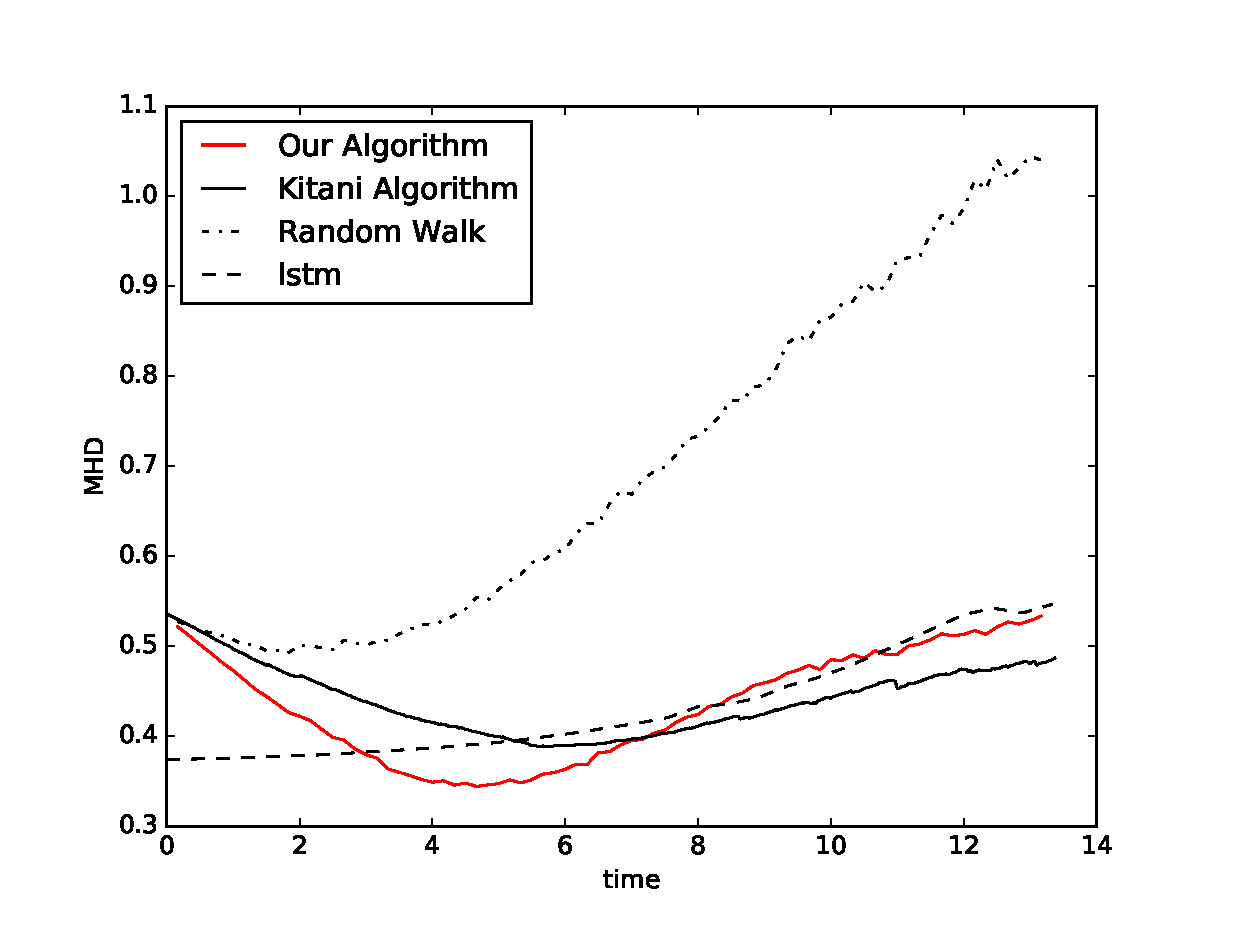
\includegraphics[width=0.6\textwidth]{figures/mhd_results.eps}
	\caption{A comparison of the Modified Hausdorff Distance from the ground truth of the pedestrian to a 1000 point samples from each distribution. The method from \cite{Alahi2016} does well at short time scales since it places a highly confident distribution at the given initial position of the pedestrian, but the method developed in this paper outperforms all others at intermediate times. At longer timescales the MHD to the trajectory of most algorithms converges. \cite{Kitani2012}, which requires the end point of each trajectory, outperforms all other algorithms which assume that the end point of the trajectory is unknown.}
   \reversemarginpar\marginnote{\#4.10}
	\label{MHD}
\end{figure}

\begin{figure}
	\centering
	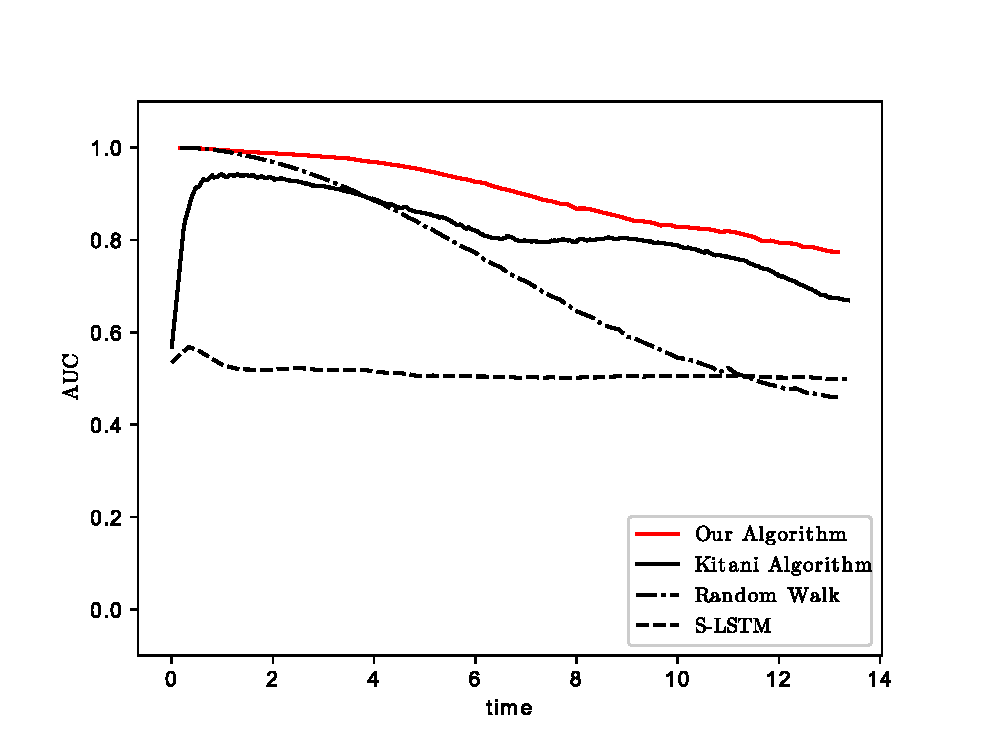
\includegraphics[width=0.6\textwidth]{figures/the_results.eps}
	\caption{A comparison of the AUC of the various algorithms. Note that the initial dip in the performance of \cite{Kitani2012} is due to their confidence in their initial estimate. We sampled the S-LSTM \cite{Alahi2016} model $100$ times to give them the best chance in this analysis \Ram{why does sampling a $100$ times give them the best chance?}, but their confidence combined with the over-reliance on social forces at moderate-to-large timescales lowered their performance.}
	\reversemarginpar\marginnote{\#4.9}
	\label{AUC}
\end{figure}

\begin{item}
\textbf{How the model can incorporate the interactions among pedestrians (i.e
group motion) and the influences from neighbouring pedestrians (for
instances such as collision avoidance)?}
\end{item}

Thank you for this insightful question. 
Since the focus of this paper was on developing a method to generate predictions at real-time for the autonomous vehicle context, we did not consider the effect of incorporating interactions between predictions. 
However, social forces are a natural avenue for future work, and so we included the following paragraph in the paper:

\response{Though including social forces into the model is outside of the scope of this paper, its incorporation could begin as follows.  
In the current motion model with a single vector field, the acceleration of the $i$th agent is given by $\ddot{x}_i = s^2 DX(x_i) \cdot X(x_i)$.  
Incorporating a social force $F_{i}$ acting on the $i$th agent can be done by instead asserting $\ddot{x}_i = s^2 DX(x) \cdot X(x) + F_i$.  
Usually $F_{i} = \sum_{j} \nabla U( x_j - x_i)$ where $U$ is an interaction potential \cite{Helbing1995}. 
The algorithms for generating real-time prediction would then generalize to this new vector-field definition.
}


\begin{item}
\textbf{Presentation and organisation
The motivation behind choosing start/end points based clustering is not
clear. Does clustering based on start/end points help to identify
different motion models? Isn't it better to cluster considering the
entire trajectory? }
\end{item}

Thank you for this relevant question.
As stated in \cite{Morris2009}, the choice of clustering technique is not nearly as important as the distance metric. 
Our success with distance functions that took a whole trajectory was limited on the data we tested and we found more success using a custom distance metric that only considered the start and end points of a trajectory as we describe in Comment \ref{distmetric} to Reviewer 1. 
We have several hypotheses as to why this is true.  
For one, the spatial scale of the data we test against showcases important features (e.g. curb cuts and storefronts), which lead to clustered start points and end points. 
Similarly, we tested against high quality data in which trajectories with irreconcilable occlusions were rare and thus could be omitted. 


\begin{item}
\textbf{Do you cluster different scenes provided in campus dataset \cite{Alahi2016} (i.e
Valley, Fangron) separately or all together? When motion models are
learnt, are they learnt in scene specific manner or altogether?}
\end{item}

Thank you for noticing that this is unclear. 
Our algorithm trains on each scene independently, so clustering, vector field learning, and learning the potential functions are all done for each scene separately. 
To make this more clear, we added the following text to the paper:

\reversemarginpar\marginnote{\#4.3}
\response{We did a 2-fold cross validation by using 20\% of the data for testing and the remainder for training within each scene. 
We learned separate collections of vector fields and model parameters for each fold on all of the four scenes on which we tested.}


\begin{item} \label{distmetric}
\textbf{The motivation behind choosing the affinity propagation clustering algorithm is not clearly stated. 
What is the distance measure used (i.e Euclidian) ? 
Not specifying such information makes reproduction of this work not feasible. }

This was an oversight on our part, thank you for noticing it. 
The distance used is a custom distance function on $\mathbb{R}^4$, which disregards the involution $(x_1, x_2, x_3, x_4) \to (x_3, x_4, x_1, x_2)$, and so does not care about parity of trajectories. 
\Ram{You are using words that roboticists do not know (e.g. involution).  
Can you please explicitly give the distance function and explain its properties and why you selected for those properties?
For example you say parity of trajectories.
What does parity mean and why is it important that the distance function ignore it?
In your response below what is $x_1,x_2,x_3,x_4$ correspond to in the scene? 
It may make more sense to use $(x_1,y_1)$ and $(x_2,y_2)$ since this is more indicative of the relationship between the points.
What is $\bf{y}$ in your definition below?
Please be more clear, again its easier for us to reduce the text then it is for us to add.}
We have included the following clarification:

\reversemarginpar\marginnote{\#4.2}
\response{We then cluster in $\mathbb{R}^4$ using Affinity Propagation \cite{FreyDueck2007} and a custom distance measure defined by $d((x_1, x_2, x_3, x_4),\mathbf{y}) : \mathbb{R}^4 \times \mathbb{R}^4 \to \mathbb{R} = \min \left\{ d_e((x_1, x_2, x_3, x_4), \mathbf{y}), d_e((x_3, x_4, x_1, x_2), \mathbf{y}) \right\}$, for the euclidean distance $d_e$. This function measures the distance between the endpoints irrespective of their ordering. The scale of the datasets we tested on had large enough spatial scale that clustering based on endpoints captured people moving from destination to destination, e.g. from a storefront to the sidewalk at the edge of a scene. On this dataset, other distance measures \Ram{are these distance functions that utilize the entire trajectory?} from \cite{Morris2009} and \cite{Lee2007} didn't \Ram{avoid contractions} identify coherent \Ram{what does coherent mean?} motion models. This is partly due to the fact that oftentimes pedestrians would take slightly different routes to get to their destination, and the cumulative effect on the distance measures is enough to hinder the clustering \Ram{what does hinder clustering mean? Please be more explicit}. }
	
\end{item}

\begin{item}
\textbf{Adequacy of Citation
I believe literature review section can be improved using a sub section
on social force models, which is extensively applied for pedestrian
trajectory forecasting. 
Helbing and Molnar, 1995; Koppula and Saxena, 2013; Pellegrini et al.,
2010; Yamaguchi et al., 2011; Xu et al., 2012; Wang et al. 2008;
Hospedales et al. 2009; Emonet et al. 2011; Yi et al. 2015.}
\end{item}

We agree that this adds to the paper, thank you for the suggestion. 
We added the following section to our literature review to reflect the relevant work:

\reversemarginpar\marginnote{\#1.1}
	\response{On the other hand, many authors have approached pedestrian forecasting by deriving their motion model from interactions between pedestrians. 
	Early work by \cite{Helbing1995} and \cite{Xu2012} describe pedestrians interactions using physically motivated methods. 
	Several models such as \cite{Yamaguchi2011}, \cite{Yi2016}, and \cite{Pellegrini2009} derive their motion models from \cite{Helbing1995} who incorporates collision avoidance through an interaction potential. 
	However this method suffers from not planning for other pedestrian'� positions at future times. 
	\cite{Emonet2011}, \cite{Hospedales2009} , and \cite{Wang2009}  all take optical flow as input.
	 \cite{Wang2009} and \cite{Emonet2011} both use variants of Hierarchical Dirichlet Processes on discretized optical flow to determine temporal motifs (i.e. classes of motion within the scene), where \cite{Hospedales2009} substitutes a Markov model. 
	 These models are not agent based, and the lack of an explicit motion model limits their predictive power. 
	 \cite{Koppula2016} predict trajectories by introducing and sampling Anticipatory Temporal Conditional Random Fields which incorporate learned affordances for humans and objects based on observed objectives within the scene. 
	 \cite{Tay2008} , \cite{Wang2008}, and \cite{Trautman2015} create agent-based models based on Gaussian Processes, though they suffer issues when trained on discretized trajectories. 
	 \cite{Alahi2016} uses Long Short-Term Memory (lstm) to learn pedestrian motion models without making assumptions about the manner in which agents will interact and is the state-of-the-art algorithm for socially based models while also having a quick run time. }

\begin{item}
\textbf{Furthermore a comprehensive review on trajectory clustering algorithms
is required. This should be used to motivate the reason of choosing
affinity propagation algorithm in section 4. 
Morris and Trivedi 2009; Giannotti et al. 2007; Lee et al. 2007;
Ester et al. 1996 }

Thank you for this suggestion and for the list of relevant titles.
 We included a note about different algorithms as well as a justification for why we chose our metric which is described in Comment \ref{distmetric} to Reviewer 1. 
 %We were unable to test against the methods of Giannotti and Ester.\Ram{why not?}.

\end{item}
\end{enumerate}


\section*{Reviewer 2}
\begin{enumerate}
\begin{item}
\textbf{Keep the good work going. Interesting approach.}
\end{item}

Thank you for the kind comments.

\begin{item}
\textbf{
Need to be clearer and
dive a little bit deeper into the technical approach. }

Thank you for this criticism. 
We hope we adequately addressed it by strengthening the description of our method for learning the motion model, as well as quantifying the way that we tested our data as is described in our responses to the suggestions by other reviewers.

\Ram{I don't think we need this addition to the text.}  
We also changed the language below to better reflect that the specific implementation we chose is an example of how to use the larger framework.

\reversemarginpar\marginnote{\#4.1}
\response{Given the model established in the previous section, we describe an implementation to showcase one way the model can be applied to observational data.}
\end{item}


\begin{item}
\textbf{
Need to use and apply more deep learning approaches such as social LSTM
or other machine methods.}

Thank you for the suggestion. 
We hope that we have addressed it by including a review of literature of social motivated models, including S-LSTM, as well as a section on how social factors can be integrated into our model. 
In addition, we compared our approach against S-LSTM in addition to the method proposed in \cite{Kitani2012}. 
The figures corresponding to the predictions of the S-LSTM model are omitted from the paper because as happened for many of the agents, the S-LSTM predictions quickly exit the bounds of the scene, and so the visualization is identically zero \Ram{I don't like this. We should include these predictions somehow anyway.}. 
We changed the subtitle of the figure to reflect this, which is shown below.

\reversemarginpar\marginnote{\#4.8}
\response{An illustration of the predictions generated by the various algorithms. In this figure, the dot is the start point of the test trajectory, the diamond is the position at time t, and the X is the end of the trajectory. The likelihood of detection is depicted using the virdis color palette. Notice that the Random Walk is imprecise, while the predictions generated by the algorithm in \cite{Kitani2012} suffer from the inability of their motion model to adequately match the speed of the agent. The algorithm from \cite{Alahi2016} quickly passes beyond the boundaries of the scene, so the plots are ommitted here.
}

\end{item}

\end{enumerate}

\section*{Reviewer 5}
\begin{enumerate}
\begin{item}
\textbf{
It would be more interesting if the authors show whether
the prediction algorithm would transfer the learned "knowledge" of
forecasting in novel scenes.}

Thank you for your comment. 
Though this was not the focus of this paper, the low-dimensional parameterization of the vector fields make transfer learning more amenable. 
As it is, this is as an immediate avenue for future work which we describe in the following addition to the text: 
\response{We also hope to do transfer learning \Ram{I flipped the previous two words.} with this model using scene segmentation from \cite{Walker2014}, as well as the semantic context descriptors and routing scores from \cite{Ballan2016} to show how vector fields can be transferred to novel scenes. It appears that the low-order parameterization of our model, and unit-length vector field assumption make it particularly amenable to the methods developed in \cite{Ballan2016}.}


\end{item}
\begin{item}
\textbf{
More statistically result is expected
rather than analyzing "four different scenes", and comparing run-time
by "averaged across several agents and scenes" (how many?).}

Thank you for noticing this oversight on our part. 
We have modified the paper in the passages listed below to clarify the list of scenes we ran in comparison, and how many agents total were run. 
The set of agents used during evaluation were the same that were used to determine run times. 
Note that we attempted to compare on all of the scenes in the Stanford Drone Dataset, but the difficulty in getting the other models to converge in a reasonable amount of time prevented us from doing so.

\reversemarginpar\marginnote{\#4.4}
\response{ Our analysis was conducted on the Coupa, Bookstore, Death Circle, and Gates scenes from the dataset from \cite{Robicquet2016}, with a total of 142 trajectories analyzed.}

\reversemarginpar\marginnote{\#4.6}
\response{The run time per frame for each algorithm was generated using the mean run time for 400 frames, averaged across all of the trajectory data used in the quality analysis.}
\end{item}

\begin{item}
\textbf{
Besides, it is better to explain the meaning of ROC and AUC in section IV.}

This is a necessary clarification, thank you for the suggestion. 
We have included a description of ROC and AUC, as well as a justification for why we chose to evaluate the methods using this criterion in our response to Comment \ref{newmetrics} for Reviewer 1.

\end{item}
\end{enumerate}

% \section*{Associate Editor?}
% \begin{enumerate}
% \begin{item}
% \textbf{The manuscript presents an interesting approach toward pedestrian
% forecasting which is quite different than current approaches.}  
% \end{item}
% \begin{item}
% \textbf{The
% presentation could be improved by providing more concrete performance
% measures and comparison with more state-of-the-art.For example newer
% models that utilize social interactions.  Please see the reviewer
% comments for more detailed recommendations.}
% Thank you for the suggestions, we feel that they have added to the quality of the paper. As stated in the individual responses to reviewers, we tested using a variant of the MHD method used in [7], and found that while we still outperformed [7] and [13] in the intermediate time scales, it didn't capture our desire to test for safety as well as proximity to ground truth as well as the AUC of the ROC curves. The plot of measured MHD is included \todo{(?)}.

% The addition of a comparison to social interaction models was very valuable, and we thank you for the suggestion. We have included a section in our literature review on these models, as well as a comparison in section IV to the S-LSTM model from [13].

% \end{item}
% \end{enumerate}
\bibliographystyle{IEEEtran}
\bibliography{references}
\end{document}